\chapter{Facility description}

    \section{Laser}

        Use section like this?

    \section{Version 1} \label{sec:design_v1}

        The design process of the first generation thruster, called Version 1 (V1), can be found in \textcite{duplayArgonLaserPlasmaThruster2024a}. It proved to be a dependable prototype, repurposed from a previous unrelated experiment. However, it presented problems that required a second generation prototype to be designed and manufactured.

        [Add short description of V1 here]

        V1 was powered by an IPG Photonics YLR-300/3000-QCW-MM-AC Ytterbium fiber laser, 

        \begin{figure}[!ht]
            \centering
            \begin{subfigure}[t]{\textwidth}
                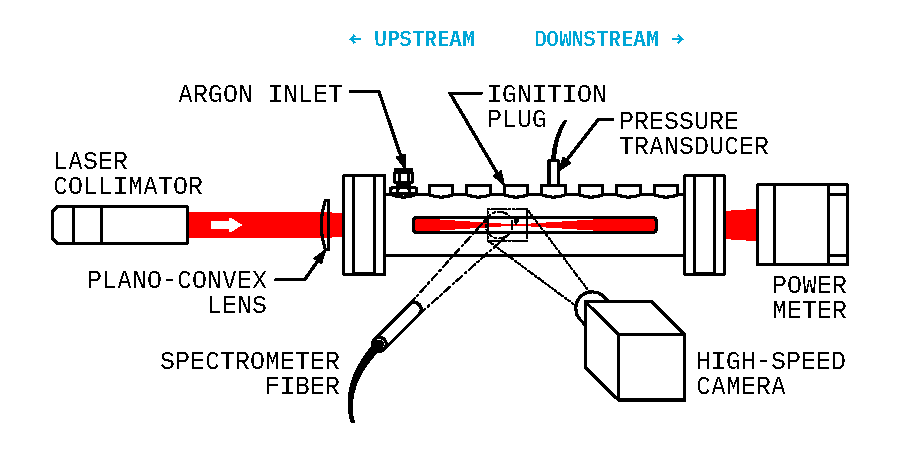
\includegraphics[width=0.85\textwidth]{assets/3 design/finalsetup_static.pdf}
                \caption{Static setup}
            \end{subfigure}
            \hfill
            \begin{subfigure}[t]{\textwidth}
                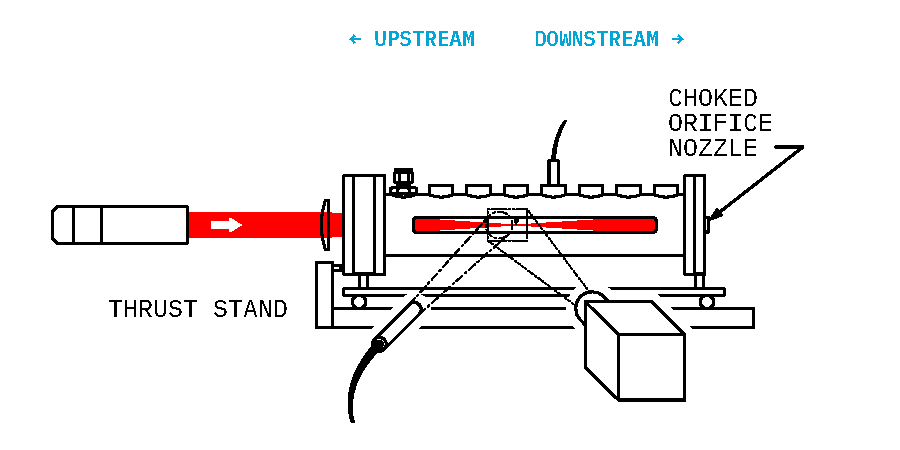
\includegraphics[width=0.85\textwidth]{assets/3 design/finalsetup_flowing.pdf}
                \caption{Flowing setup}
            \end{subfigure}
            \caption{V1 LTP thruster}
            \label{fig:V1 setup}
        \end{figure}

        \subsection{Capabilities}

            298 recorded pulsed laser shots were conducted with V1, exploring the power-pressure threshold, wire initiation and spark initiation.

        \subsection{Issues}

            Too heavy -> too much friction on rail for thrust tests. This was mitigated in part by a rope system.

            Critically, rubber seals were exposed to laser path during continuous lasing with a lower focal length lens (picture), severely burning them in the only CW test conducted. A shorter test section designed for a \qty{100}{mm} focal length lens would solve this.







    \section{Version 2} \label{sec:design_v2}

        To improve upon the V1 facility, an entire redesign was done. This resulted in the much smaller Version 2 (V2) purpose-built LTP thruster at the end of April 2024.

        \subsection{Requirements}

            The following requirements were developed for the design of the V2 thruster. The objective was to detect a measurable difference in thrust between an argon cold gas thruster and an argon “hot gas” thruster, heated by a laser supported plasma (LSP).

            \begin{enumerate}
                \item Laser thruster
                \begin{enumerate}
                    \item A \qty{300}{W} Continuous Wave (CW) \qty{1070}{nm} laser shall sustain the plasma (Nominal power \qty{300}{W}, actual max power \qty{350}{W})
                    \item The thruster shall have a minimum safe “hot” operation time of \qty{30}{s}
                    \begin{enumerate}
                        \item In the event of failed LSP initiation, the thruster shall safely absorb the total laser power for at least \qty{10}{s}
                    \end{enumerate}
                    \item An optical path shall be present to let the laser into the thruster, utilizing a \qty{100}{mm} focal length lens at minimum and a collimated beam with a maximum diameter of \qty{30}{mm}
                    \begin{enumerate}
                        \item The optical components shall not be damaged by the laser flux
                    \end{enumerate}
                    \item Argon shall be used as the working fluid
                    \begin{enumerate}
                        \item The argon feed gas shall be at room temperature
                    \end{enumerate}
                    \item A gas feed path shall bring argon gas into the thruster
                    \begin{enumerate}
                        \item The gas feed shall be choked at the thruster inlet
                        \item The gas feed shall be evenly distributed in the thruster
                    \end{enumerate}
                    \item The mass flow rate of the argon gas shall be measured and controlled by interchangeable upstream choked orifices
                    \item The maximum allowable operating pressure (MAOP) of the thruster shall be 50 bar
                    \begin{enumerate}
                        \item The nominal pressure of the thruster shall be 25 bar
                    \end{enumerate}
                    \item A converging-diverging exhaust nozzle shall be designed to accelerate the gas to a supersonic speed
                    \begin{enumerate}
                        \item The nozzle shall be easily changeable
                    \end{enumerate}
                    \item A 1/8" NPT port for a pressure transducer shall be present along the thruster
                    \item An optical port shall be present for spectrometry measurements of the plasma
                    \item The thruster shall be installed on a thrust stand (See section 3. Thrust stand)
                \end{enumerate}
                \item Initiation system/electrical
                \begin{enumerate}
                    \item The LSP shall be ignited by an electrical spark
                    \item The spark gap shall be measurable, controllable, and repeatable
                    \item The spark shall be generated by an AEM 30-2853 High Output Smart Coil, supplying \qty{41}{kV} with up to \qty{118}{mJ}
                    \item All parts of the thruster and thrust stand shall be directly or indirectly connected to a common electrical ground
                \end{enumerate}
                \item Thrust stand
                \begin{enumerate}
                    \item The thrust stand shall measure thrust on the order of \qtyrange{0.1}{5}{N}
                    \item The thrust stand shall minimize friction losses
                    \item The thrust stand shall be securely fixed using standard optical breadboard mounting hardware
                \end{enumerate}
            \end{enumerate}

            With these requirements, preliminary geometric dimensions of the V2 thruster could commence. It was expected to be much smaller than V1, as the goal was to isolate the LSP region and increase heat flux to the gas.

        \subsection{Sizing the double choked LTP thruster} 

            When adding energy to the thruster chamber with a laser, it is useful to choke the inflow upstream of the chamber. Indeed, this keeps the $P_0$ and $\dot{m}_\mathrm{in}$ constant, so the increase in chamber pressure can be interpreted as a measure of energy deposition (as was discussed in \autoref{chp:models}). The second choke happens at the nozzle to accelerate the hot gas to a supersonic speed. Therefore, this configuration is double choked, a classic problem in compressible fluid mechanics.
            
            The starting assumptions were the following: a \qty{300}{W} power input (the laser) supplies energy to an LTP experiment that has an internal pressure of \qty{25}{bar}, with a \qty{50}{bar} feed pressure. It is required that the hot gas operation (laser on) increases the gas' exit velocity to twice that of the cold gas operation (laser off). We will determine the gas mass flow rate and the diameter of the two orifices needed to choke the flow.

            \begin{figure}[h]
                \centering
                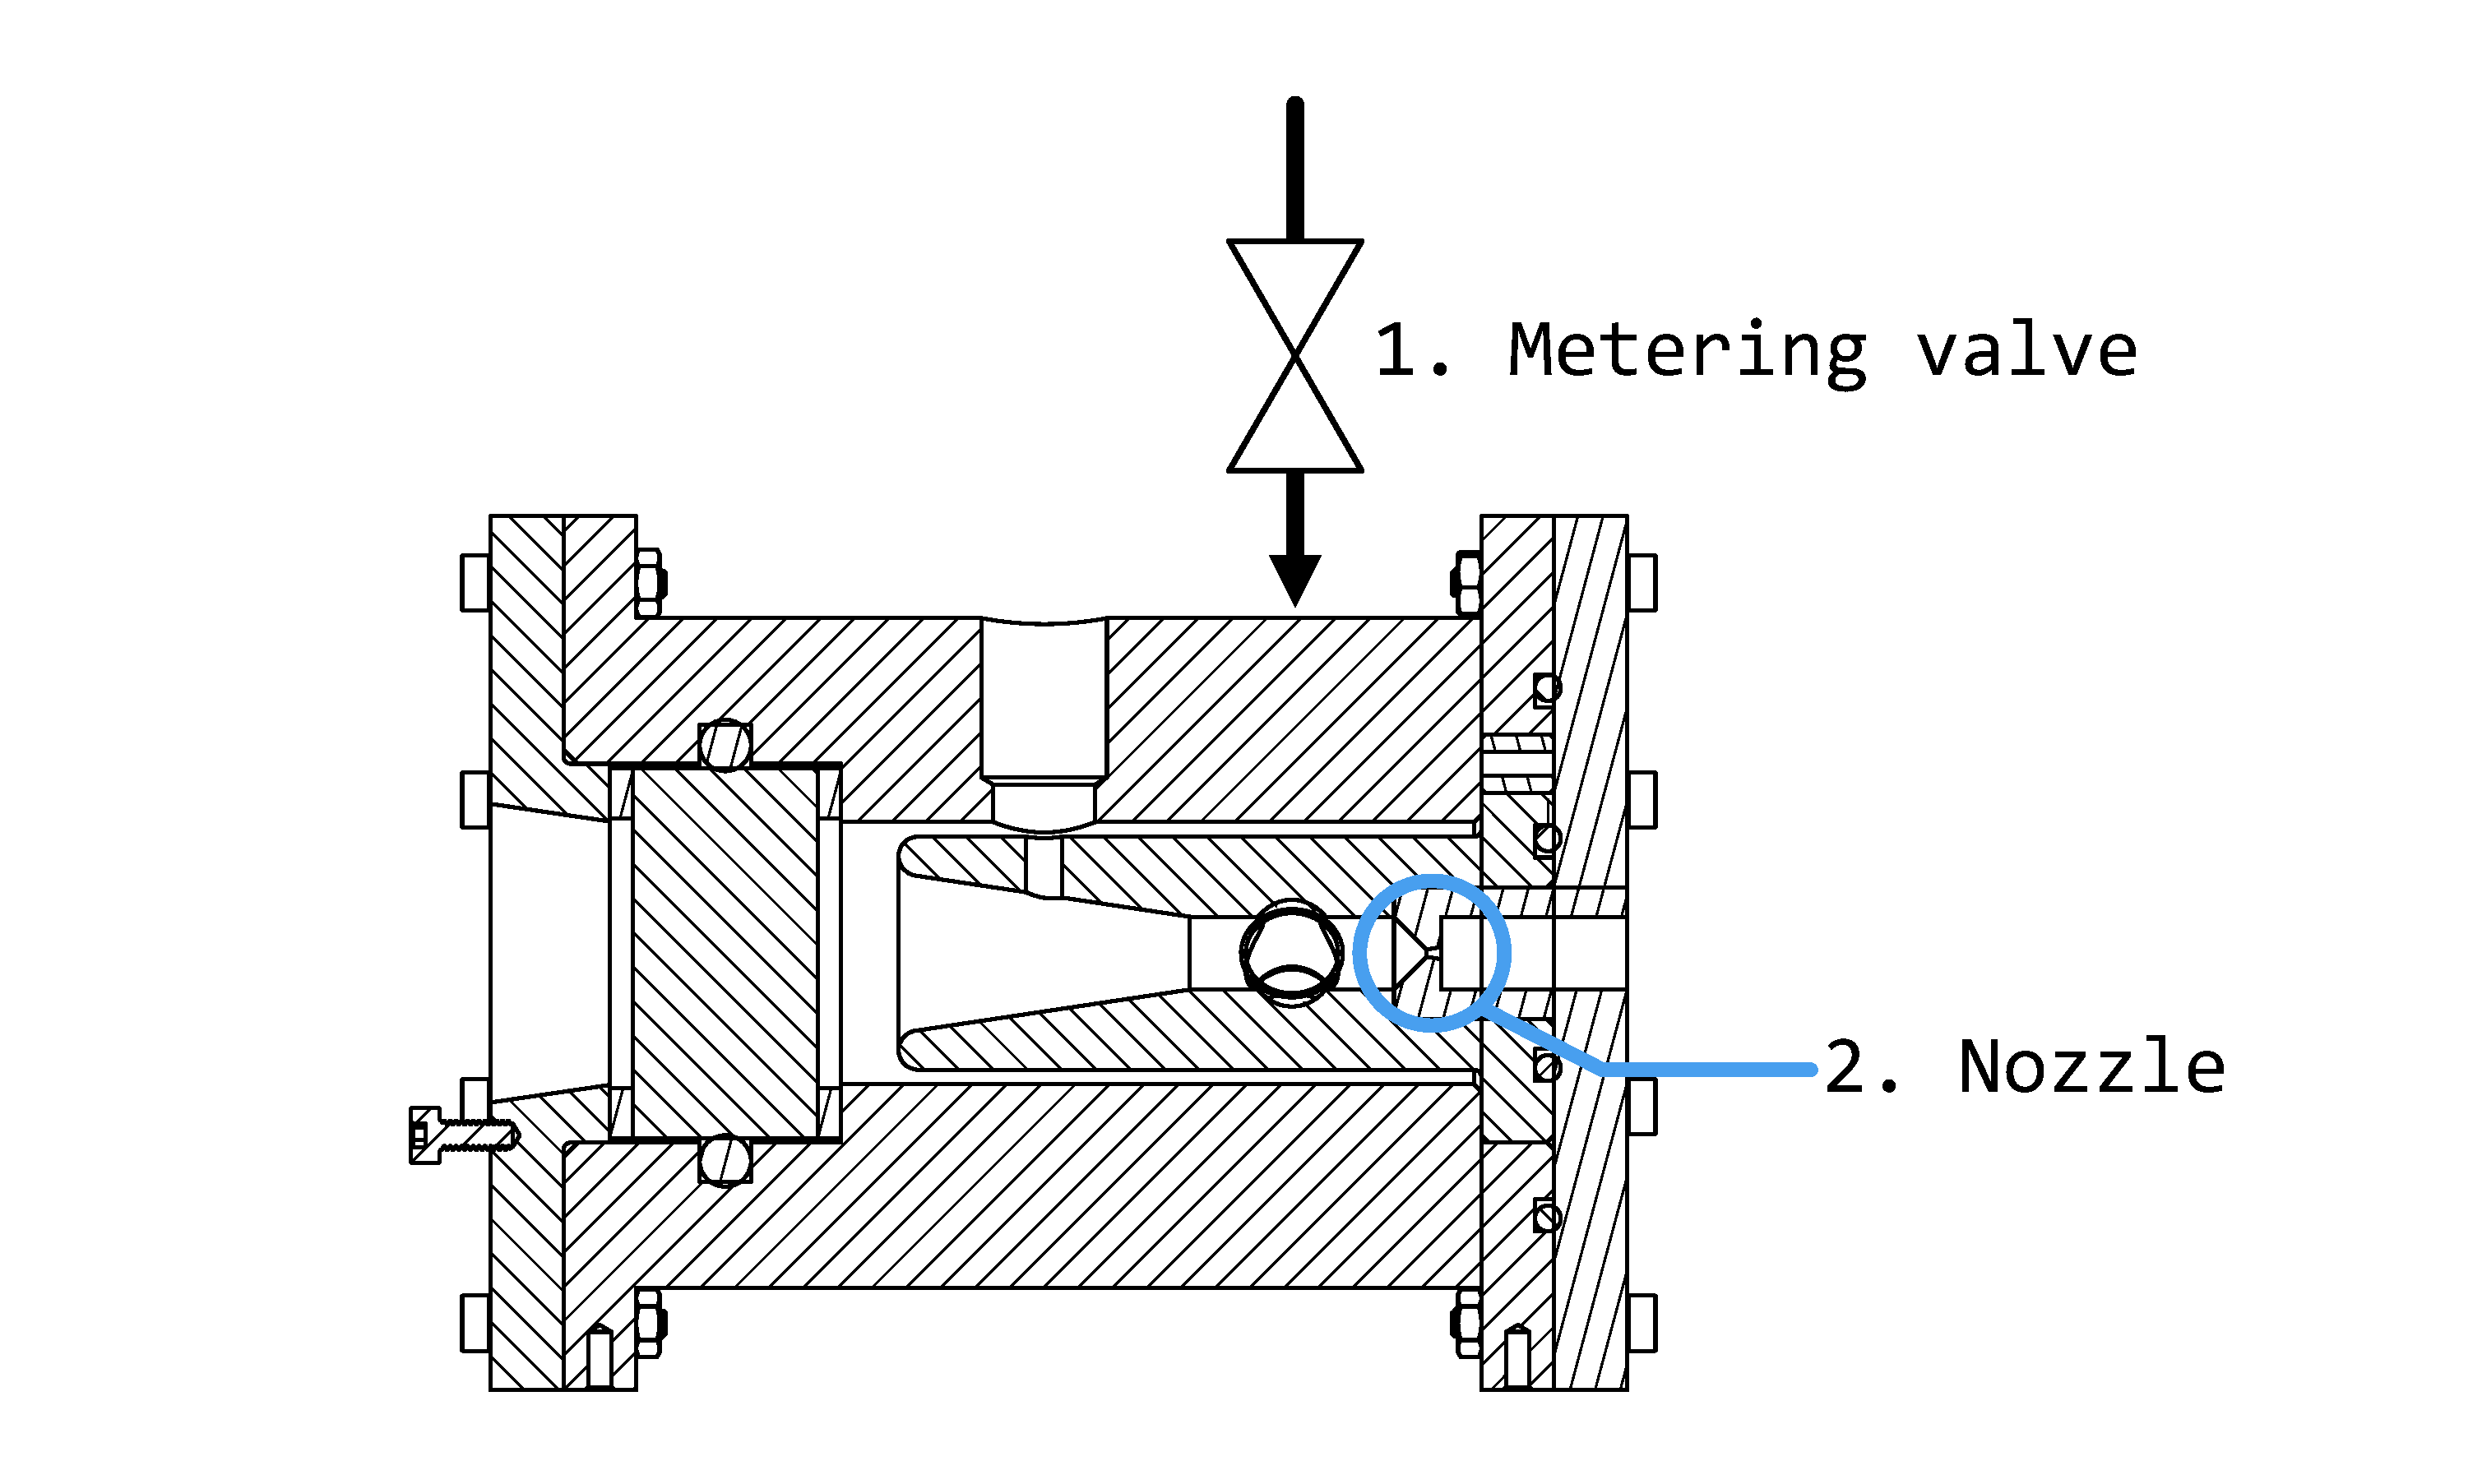
\includegraphics[width=0.8\linewidth]{assets/3 design/Double choked LTP thruster.pdf}
                \caption{Cutaway of a double choked LTP thruster showing both choking orifices: the metering valve and the nozzle.}
                \label{fig:double choke sizing}
            \end{figure}
            
            Starting with a cold gas thruster using argon, the speed of sound ($c_0$) is \qty{323}{m/s}. This is at ambient temperature (\qty{300}{K}), as we have no laser energy to heat the gas in this case. With a nozzle, the gas is accelerated to approximately twice this speed. The $v_\mathrm{exit}$, which is our main performance parameter, is therefore \qty{646}{m/s}.
            
            Laser on (hot) operation will now be examined. Taking the previous $v_\mathrm{exit}$ and ionizing the whole flow, it is posed that our efficiency is doubled. This gives a $v_\mathrm{exit}\approx \qty{1300}{m/s}$. What nozzle throat size is necessary for this $\dot m$ with $p_\mathrm{chamber} = \qty{25}{bar}$? We know that $\mathrm{MW_{Ar}} = \qty{40}{g/mol}$. The speed of sound is $c = \sqrt{\gamma R T}$. As we want to double the speed of sound, we are multiplying the temperature by 4.
            \[\text{Power} = \dot m (h_2-h_1)
            = \dot m c_p (T_2-T_1)\]
            Using a constant $c_p$ of argon of \qty{0.520}{kJ.kg^{-1}.K^{-1}}, the calculated $\dot m$ is \qty{0.641}{g/s}.
            
            Fliegner's formula describes the mass flow rate of an isentropic flow:
            \[\frac{\dot m}{A} = p_0\sqrt{\frac{\gamma}{T_0 R}}\frac{M}{(1+\frac{\gamma-1}{2}M^2)^{(\frac{\gamma+1}{2(\gamma-1)})}}\]
            With $\gamma = \frac{c_p}{c_v} = 1.666$ for argon and choked flow at the nozzle, the area and the diameter of the circular nozzle are \qty{0.176}{mm^2} and \qty{0.473}{mm}, respectively. These calculations can be repeated for the feed orifice, with the same $\dot m$, a pressure of \qty{50}{bar} and ambient temperature. This gives us an orifice size of about 0.2 mm.
        
        \subsection{Additional V2 systems}
            
            Static pressure testing up to \qty{75}{bar} for \qty{25}{minutes} was completed successfully [HOWEVER]

            \subsubsection{Electrodes}
                The \qty{44}{kV} wire having burst during pressure tests, different electrodes were necessary. Molded dielectric epoxy (Stycast ES 1001 [LINK to website]) around an industrial sewing needle core was chosen, as it was economical and the outer diameter of the electrodes could be precisely controlled by sanding the surface of the set epoxy. Molds were 3d printed and Mann Ease Release\texttrademark 300 was applied to all their inside surfaces.

                \begin{figure}[!ht]
                    \centering
                    \begin{subfigure}[t]{0.30\textwidth}
                        \centering
                        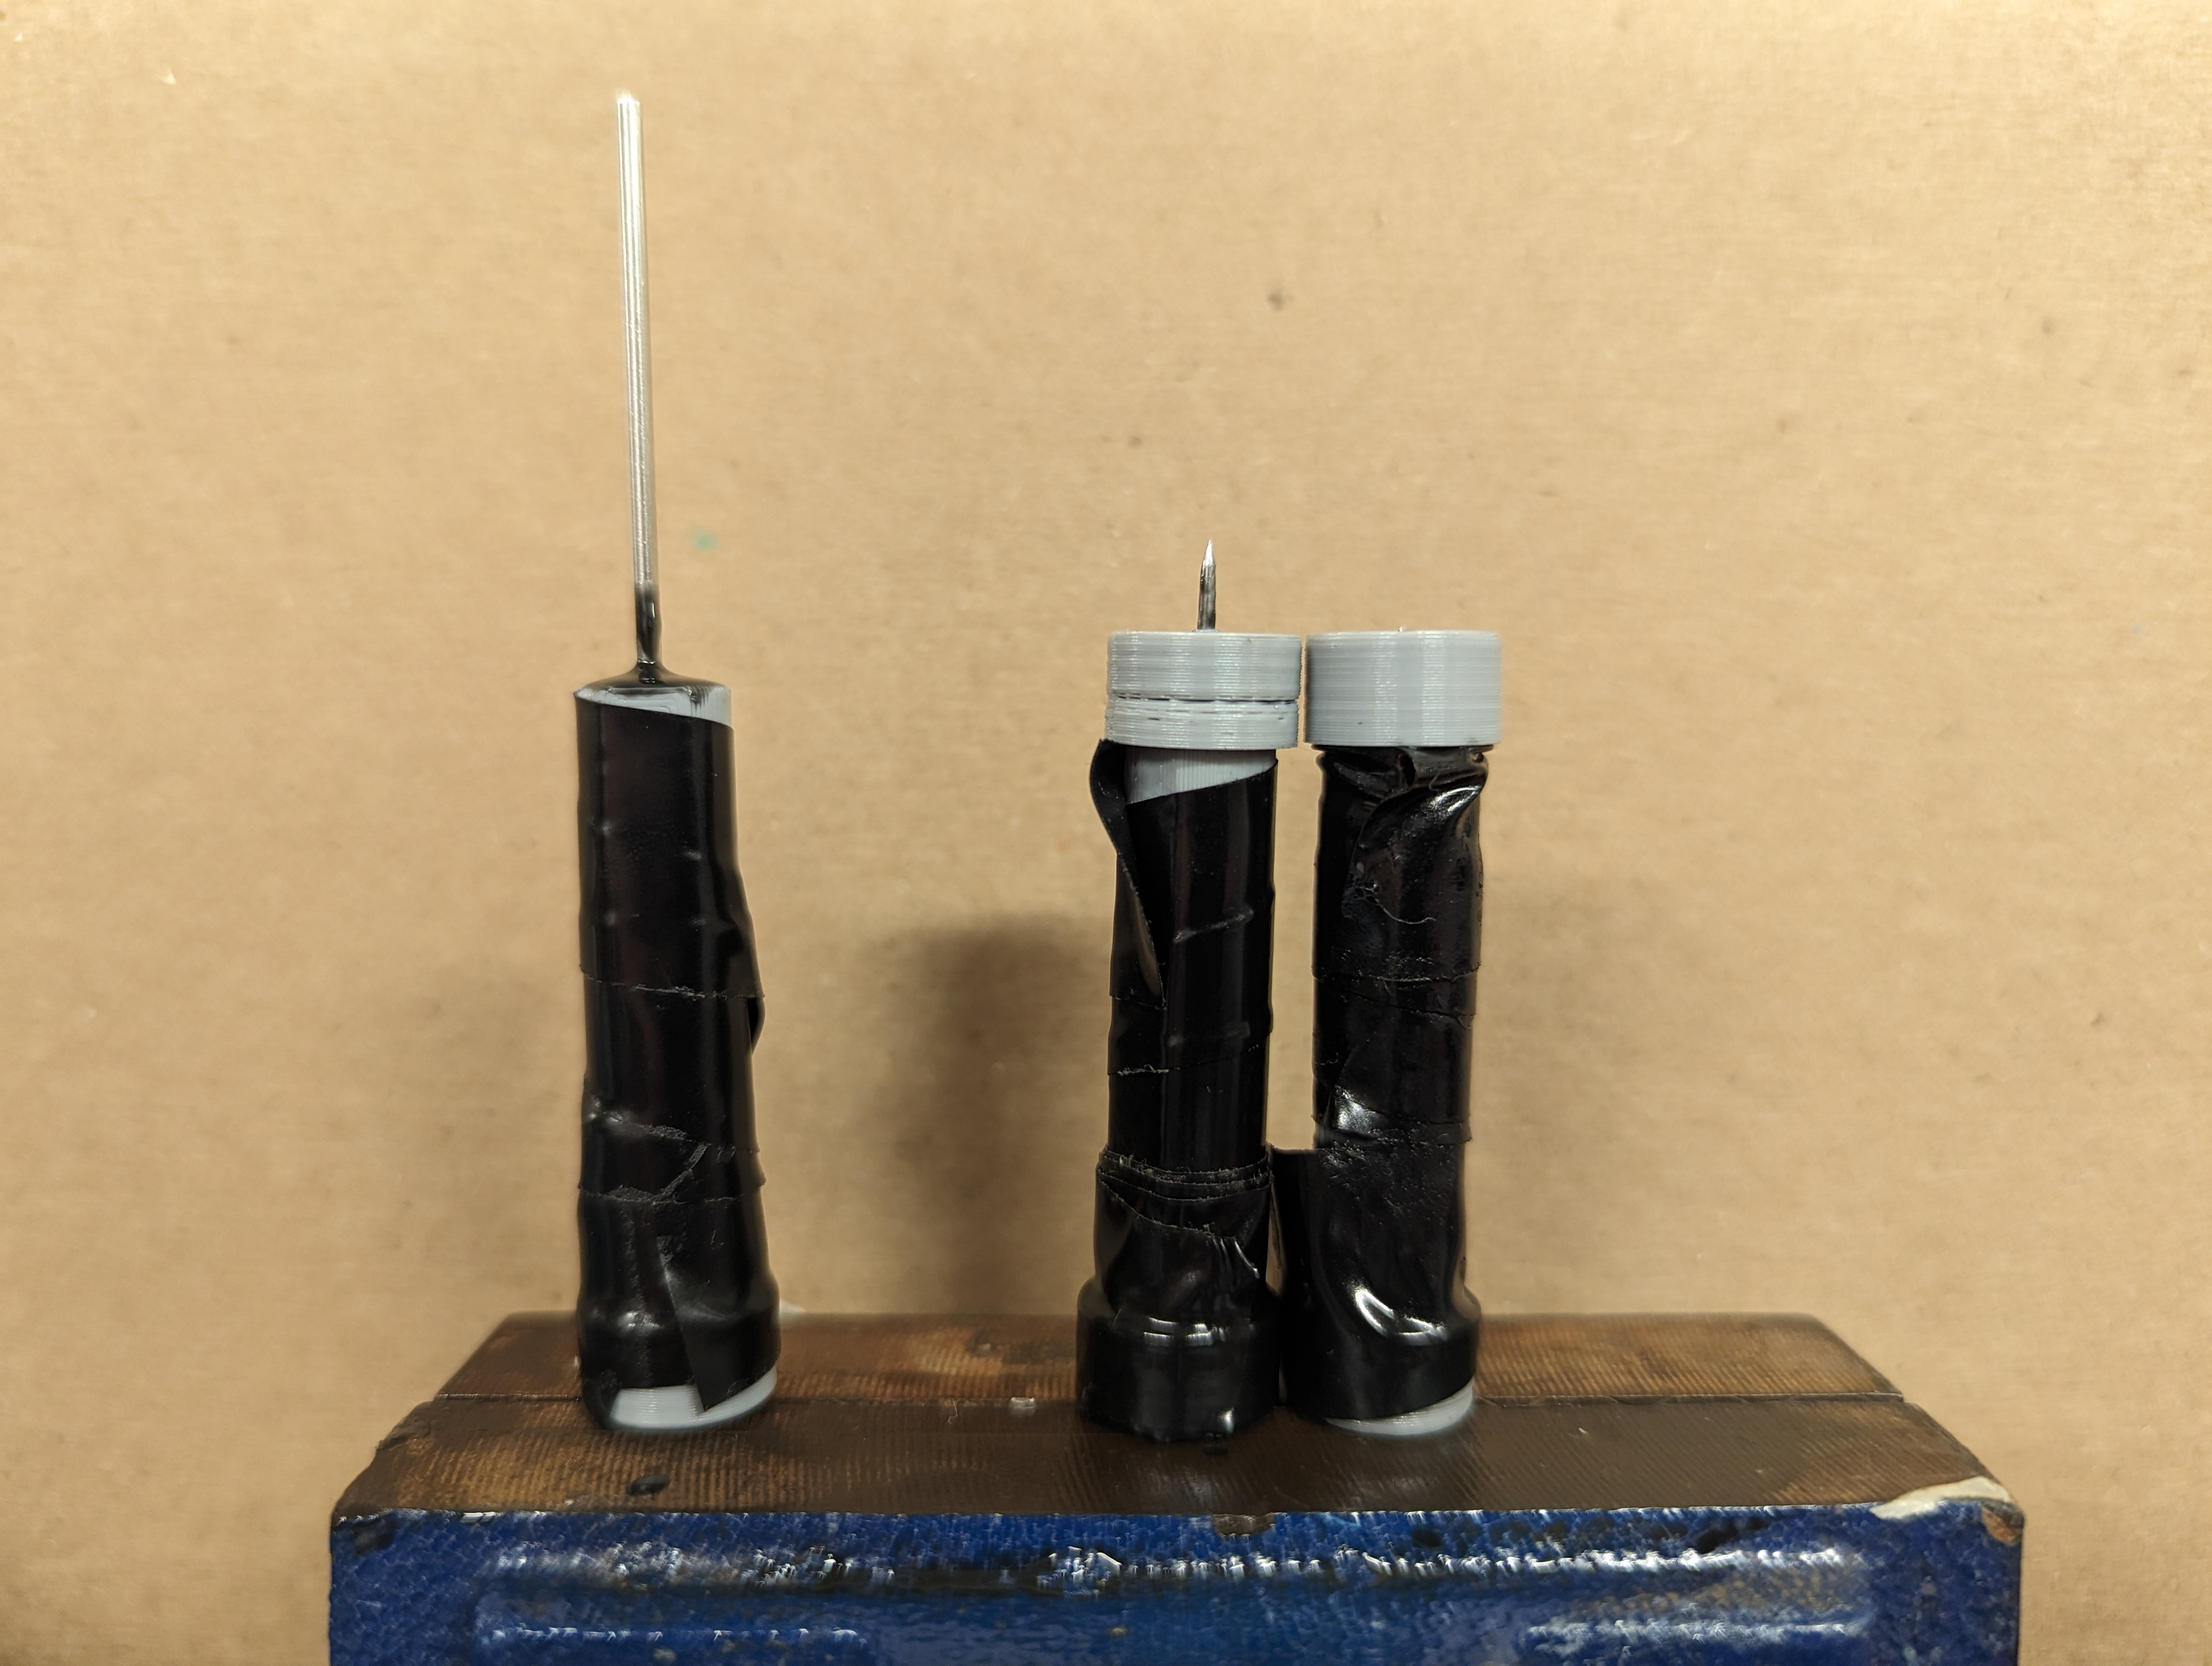
\includegraphics[width=\textwidth]{assets/3 design/Molds.jpg}
                        \caption{Molds with steel needle core in place}
                    \end{subfigure}
                    \hfill
                    \begin{subfigure}[t]{0.30\textwidth}
                        \centering
                        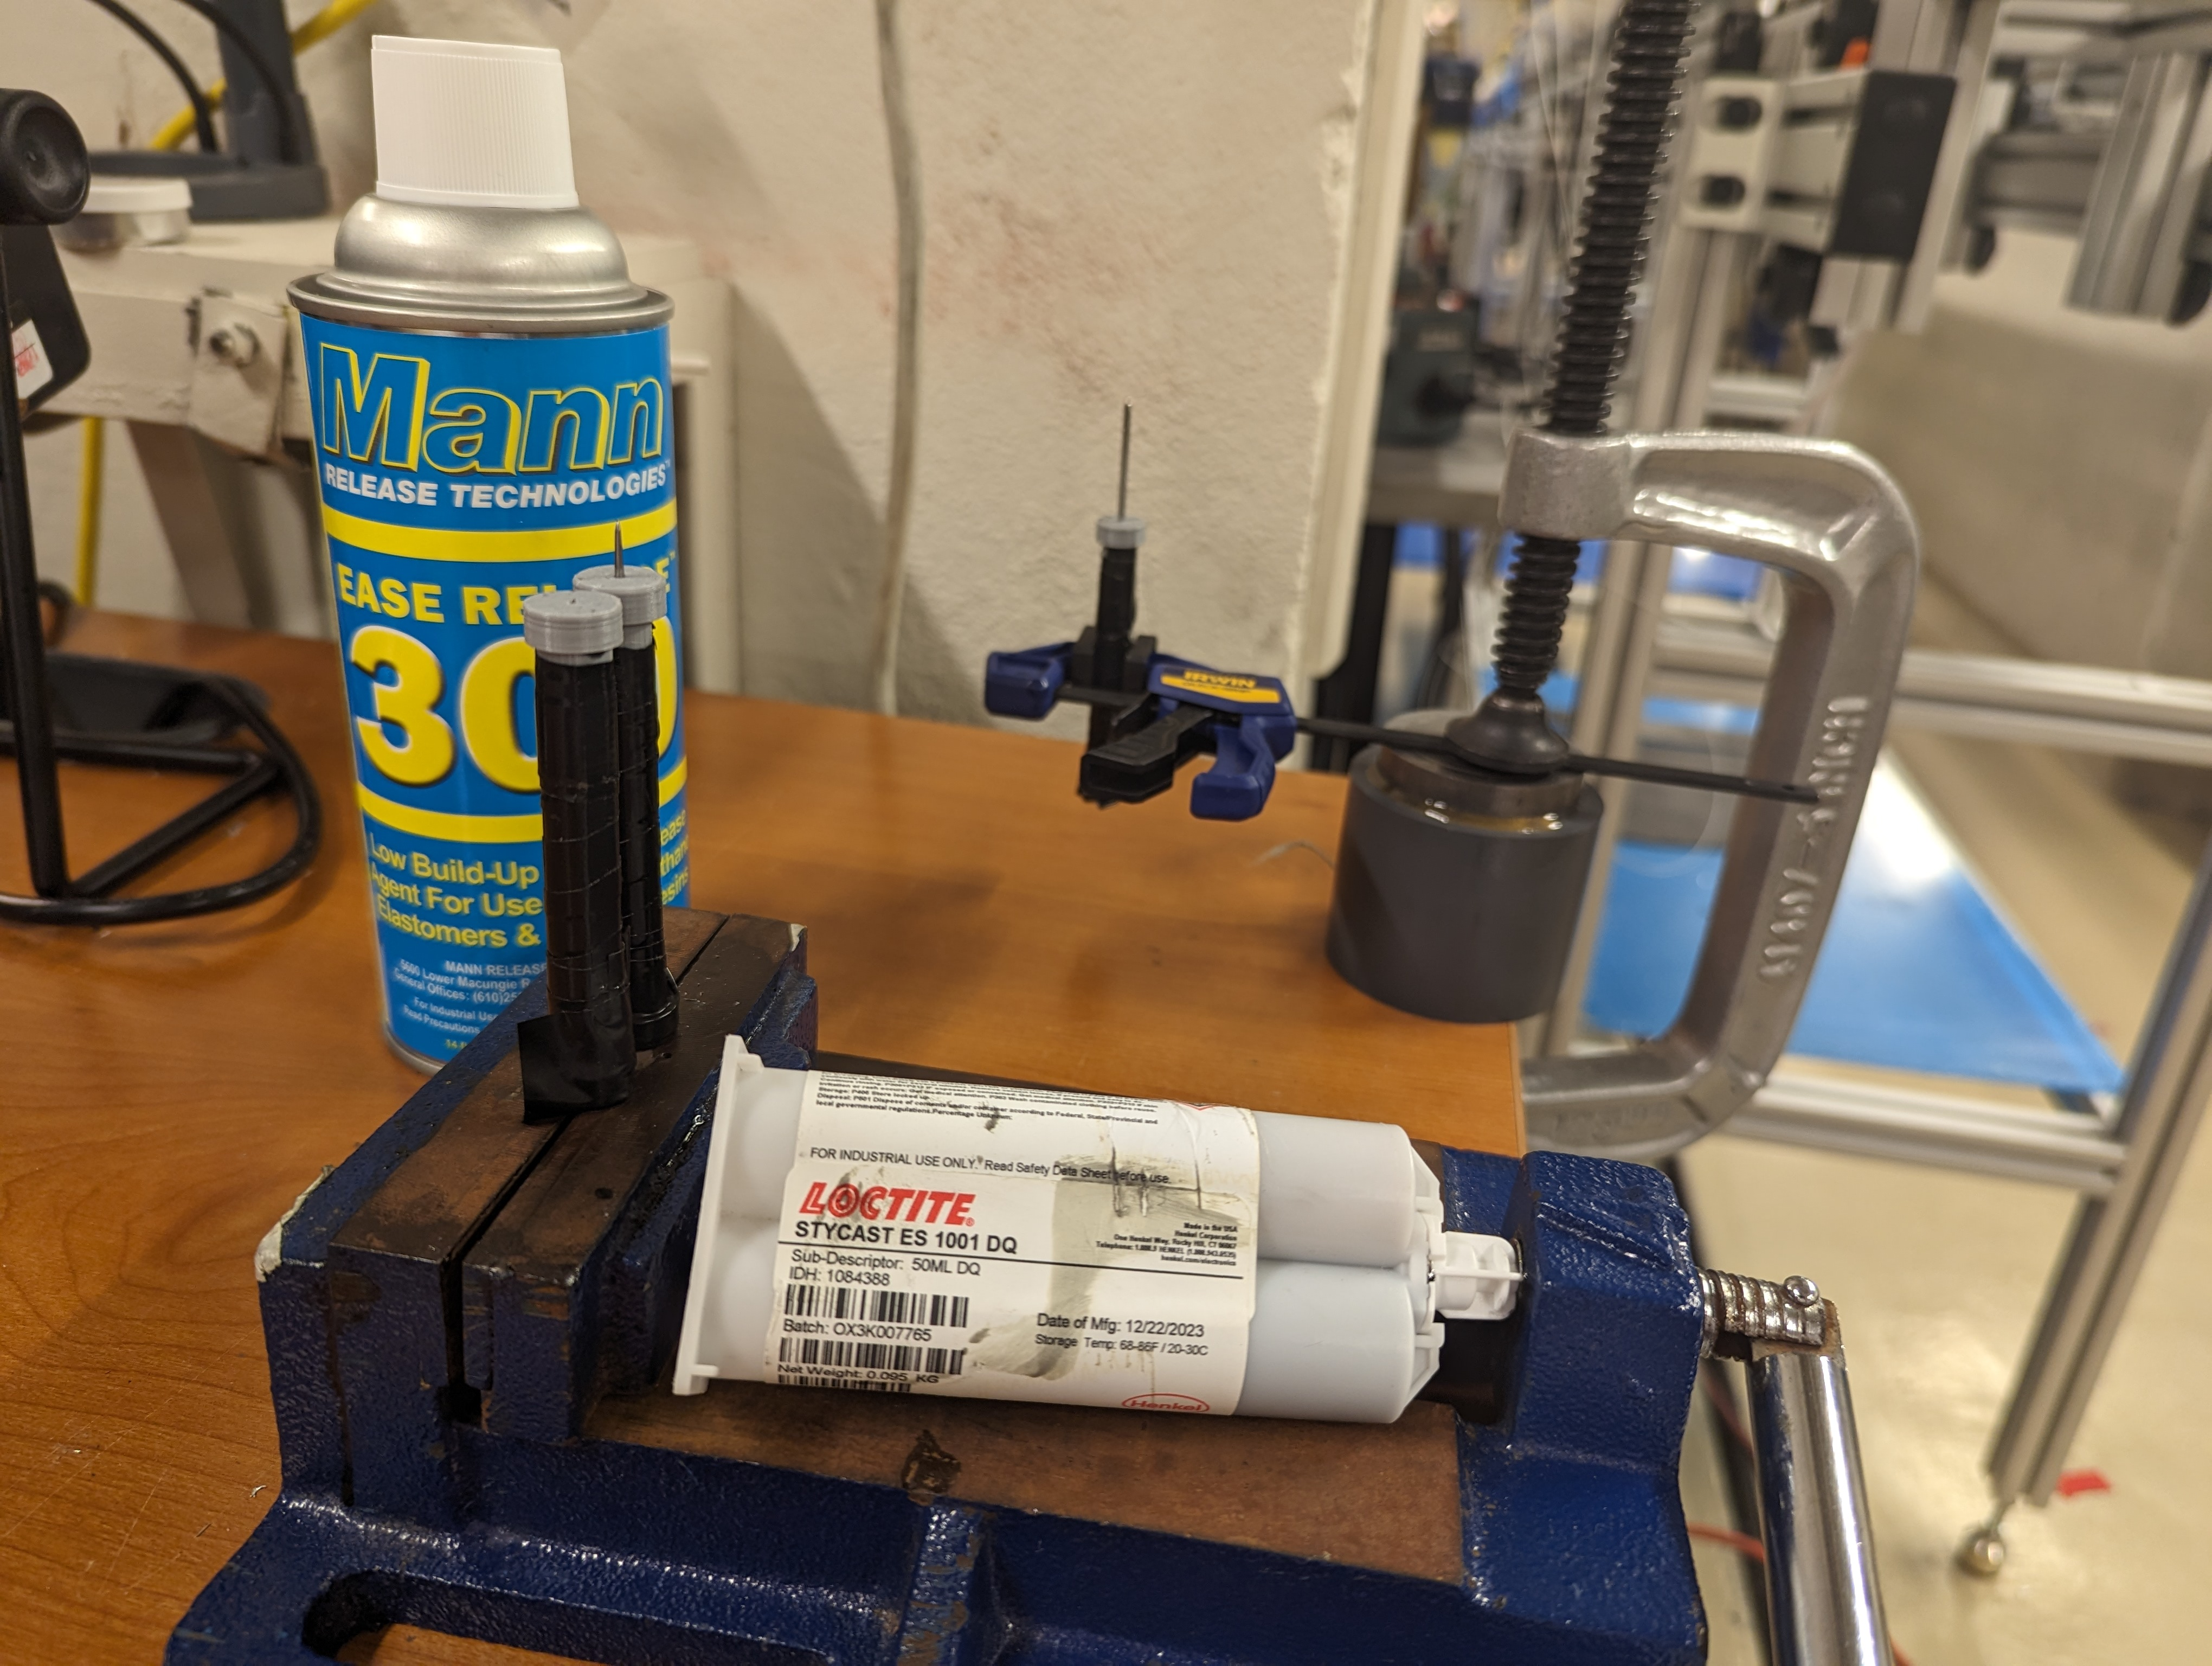
\includegraphics[width=\textwidth]{assets/3 design/Mold process.jpg}
                        \caption{Molding process}
                    \end{subfigure}
                    \hfill
                    \begin{subfigure}[t]{0.30\textwidth}
                        \centering
                        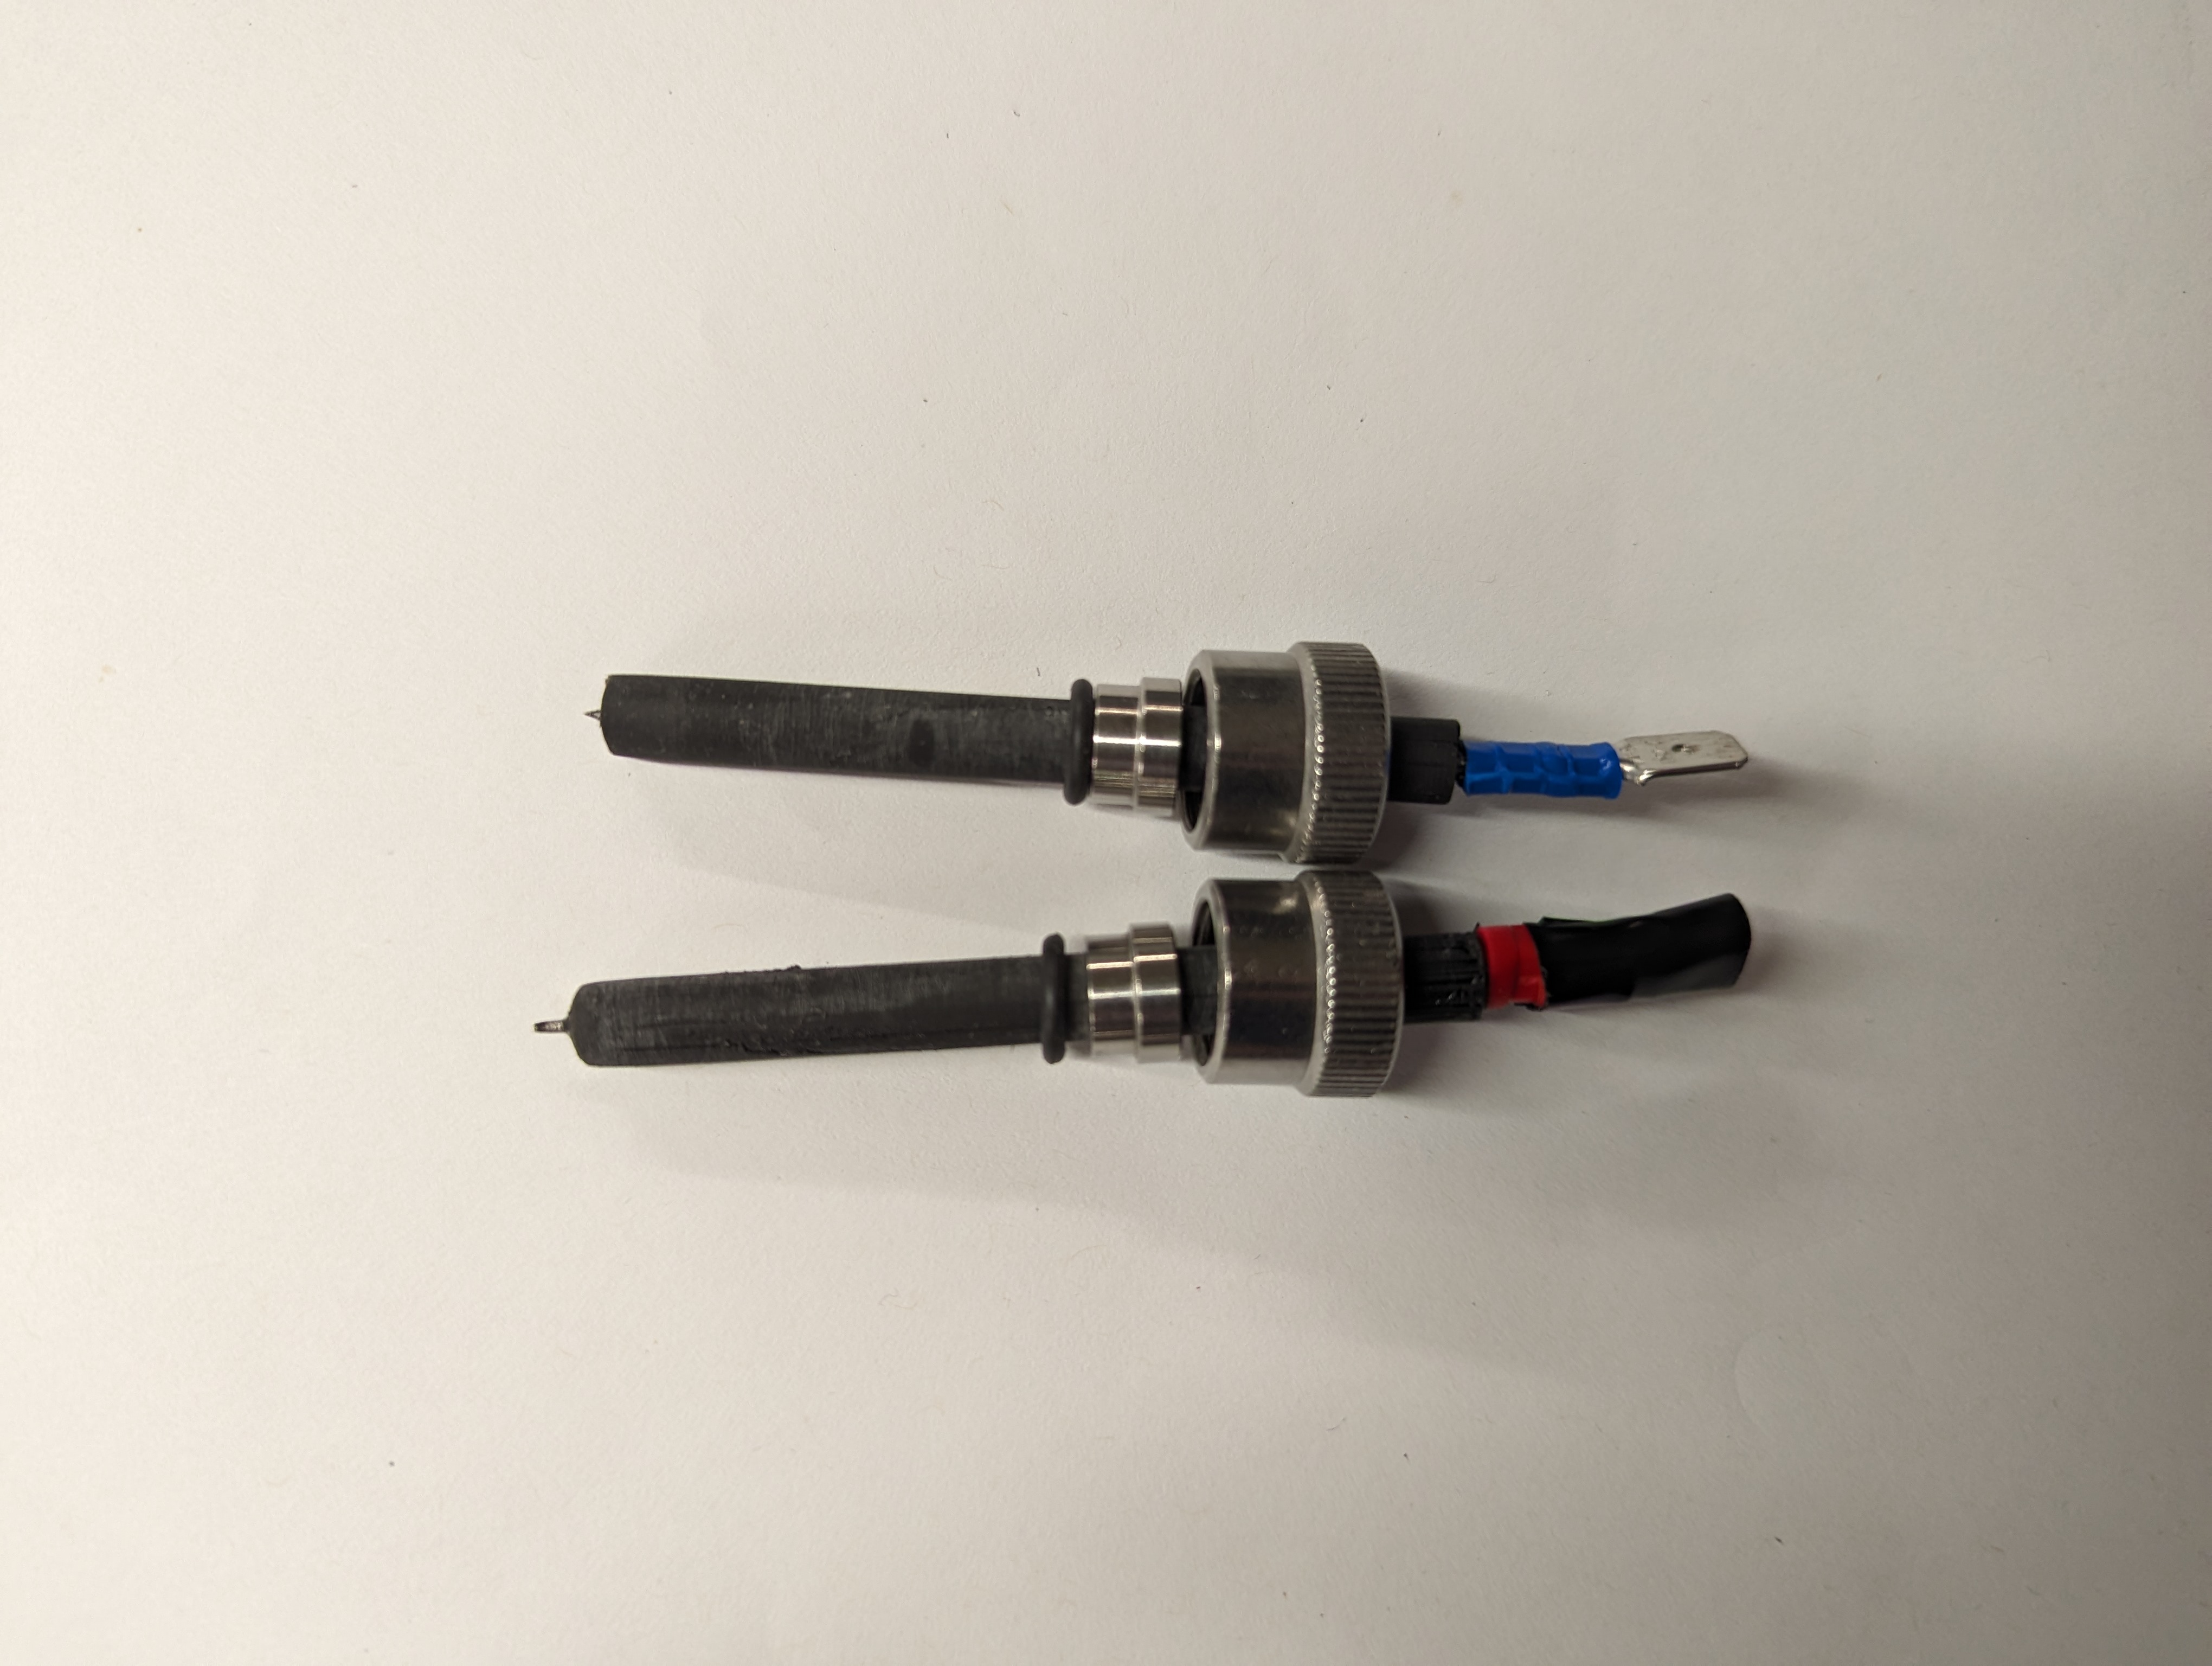
\includegraphics[width=\textwidth]{assets/3 design/V2 electrodes.jpg}
                        \caption{Assembled electrodes with Ultra-Torr cap and electrical connectors}
                        \label{fig:Assembled electrode}
                    \end{subfigure}

                    \caption{Electrode manufacturing process}
                \end{figure}

                The electrodes were then sanded down to fit tightly into Ultra-Torr vacuum connectors [link to swagelok and part number]. Although these connectors were not designed for high pressure, previous experience has shown that they are appropriate up to about \qty{20}{bar} of internal pressure if tightened enough.

                The result is presented in \autoref{fig:Assembled electrode}.

                Once installed in the V2 thruster, the electrodes were pushed into contact with each other and the Ultra-Torr connectors tightened. Statically pressurizing V2 to \qty{20}{bar} was enough to slightly separate the electrodes from one another. [add text for flow testing?]
    
    \section{Optics design}
                
                Due to the low continuous laser power compared to experiments in the literature, increasing the laser flux with small a focus is critical.

                Two ways can be used to calculate the spot size of a laser. Firstly, ray tracing software such as WinLens calculate the geometry of paraxial \footnote{Rays having small angles and distances to the optical axis} rays and show the path of these rays at the focus. Secondly, this equation \cite{LaserSpotSize} can be used: (ideal?)
                
                \[
                \text{Spot size}(mm) = \frac{4 \times \text{Focal length}(mm) \times \text{Wavelength}(mm) \times M^2}{\pi \times \text{Beam diameter at lens}(mm)}
                \]

                The beam propagation factor $M^2$ is a scale to measure beam quality. A diffraction-limited Gaussian beam has the minimum $M^2$ of 1 \cite{hechtUnderstandingLasersEntry2019}. 
                
                The YLR-300/3000 laser has a BPP of \qty{2}{mm.mrad} [Refer to appendix laser's data sheet].

                
                
                It is also implemented in WinLens, but is not based on ray tracing.

                The following spot diagrams were produced with WinLens. Note the difference in scales and spacing used throughout.

            

                \begin{table}[!ht]
                    \centering
                    \caption{Simulated focal length and spot diameter of various lens assemblies in WinLens3D. Laser flux is also calculated for \qty{300}{W} of incident power}
                    \label{tab:laser flux}
                    \begin{tabularx}{\textwidth}{@{}lX<{\raggedright}X<{\raggedright}X<{\raggedright}X<{\raggedright}@{}}
                    \toprule
                    Lens & Nominal focal length (\unit{mm}) & Focal length at \qty{1070}{nm} (\unit{mm})& Beam diameter at focus (\unit{mm}) & Laser flux at \qty{300}{W} (\unit{W/cm^2}) \\ \midrule
                    Single & 125           &  122   &    0.0863 ?  0.20?     &  \\
                    Single & 100           &  93   &    0.20   &  \\
                    Double & 500, 150      &  110    &    0.08   &  \\
                    \bottomrule
                    \end{tabularx}
                \end{table}

                (Maybe compare with minimum maintenance intensity of previous literature)

                In a two element system, the longest focal length lens should be placed first, as the diameter of the beam entering the second lens is maximized. However, it is placed after here because it is impossible to mount before. The difference in spot size is acceptable. [maybe compare?]

                Practical considerations for experiments are the following. When aligning the laser with the red visible guide beam, chromatic abberations [\dots] \cite{hechtUnderstandingLasersEntry2019}.

                The LSP will also be formed upstream of the laser focus when there is no gas flow. Therefore, the focus needs to be slightly after the ignition system. [does this change with flowing LSP?]